%!TEX root = ../thesis.tex
%*******************************************************************************
%*********************************** Seventh Chapter *****************************
%*******************************************************************************

\chapter{Centre Vortex Visualisations}
\ifpdf
    \graphicspath{{Chapter7/Figs/Raster/}{Chapter7/Figs/PDF/}{Chapter7/Figs/}}
\else
    \graphicspath{{Chapter7/Figs/Vector/}{Chapter7/Figs/}}
\fi

In previous chapters we have motivated the significance of centre vortices in QCD through the calculation of the gluon propagator. Although we can predict many of the properties of vortices through calculation, these properties can also be explored through visualisations of the lattice. To this end, in this chapter we present a novel visualisation technique that allows us to view thin centre vortices on the lattice through the use of three-dimensional (3D) models.

\section{Time Slices}
As the lattice is a four-dimensional hypercube, we visualise the centre vortices on 3D slices. The choice of dimension to take slices along is irrelevant in Euclidean space, so we choose to take slices along the $x$-axis, resulting in $N_x$ slices each with dimension $N_y\times N_z\times N_t$. This choice of axis to slice along allows for the largest volume per slice.  However, the transition between slices is best thought of as `stepping though time', so we re-label our coordinates such that each slice is a snapshot at fixed $t$, with local coordinates $(x,y,z)$. Within each slice we can visualise all vortices associated with an $x-y$, $x-z$ or $y-z$ plaquette by calculating $P_{x\,y}(\bf{x})$, $P_{y,z}(\bf{x})$ and $P_{z,x}(\bf{x})$ for all $\bf{x}$ in the slice. These vortices will be referred to as the `space-oriented' vortices, as they are fixed in time. The plaquettes are evaluated on a centre projected configuration, so $P_{\mu\nu}\in \lbrace -1,\,0,\,+1\rbrace$. For a $+1$ vortex, a blue jet is plotted piercing the centre of the plaquette, and for a $-1$ a red jet is plotted. The direction of the jet is set according to a right-hand rule, such that
\begin{enumerate}
\item $P_{x\,y}=\pm 1\implies \pm\hat{z}$ direction.
\item $P_{y\,z}=\pm 1\implies \pm\hat{x}$ direction.
\item $P_{x\,z}=\pm 1\implies \mp\hat{y}$ direction,
\end{enumerate}
An example of this plotting convention is shown in Fig.~\ref{fig:SpacialVortices}.\\

{\centering
\begin{figure}[ht]
  \begin{subfigure}[b]{0.5\textwidth}
\begin{tikzpicture}[scale=1]
\begin{scope}[very thick,decoration={
    markings,
    mark=at position 0.5 with {\arrow[scale=2]{stealth}}}
    ] 
  % bottom right to top right                    x,y start of line    label  x,y end
  \draw[line width=1.0,postaction={decorate}](1.5,-1.5)-- node[left]{$Z_y(n+\hat x)\ $} (3.25,1.5)node(g){};
  % top right to top left
  \draw[line width=1.0,postaction={decorate}](3.25,1.5)-- node[above]{${}\ \ Z_x^*(n+\hat y)$} (-1.5,1.5);
  % top left to bottom left
  \draw[line width=1.0,postaction={decorate}](-1.5,1.5)-- node[left]{$Z_y^*(n)$}(-4,-1.5);

  % Jet triangle
  % bottom left	
  \draw (-0.3,-2) node(a){}
  -- (0.1,-2) node(b){}   % bottom right
  -- (-0.1,2) node(c){}   % top
  -- cycle;               % complete
  \fill[blue] (a.center) -- (b.center) -- (c.center);
  
  % bottom left to bottom right
  \draw[line width=1.0,postaction={decorate}](-4,-1.5)-- node[above]{$Z_x(n)$}(1.5,-1.5)node(f){};
  
  % Coordinate axes       arrow head          x,y start -- x,y finish [position] label
  %\draw[line width=1.0,-{Latex[length=2mm]}](3.5,0)--(4.5,0.0)node[right]{\large $x$};
  %\draw[line width=1.0,-{Latex[length=2mm]}](3.5,0)--(3.9,0.8)node[right]{\large $y$};
  %\draw[line width=1.0,-{Latex[length=2mm]}](3.5,0)--(3.5,1.0)node[above]{\large $z$};
  \end{scope}
\end{tikzpicture}
  
  \end{subfigure}             
  \begin{subfigure}[b]{0.3\textwidth}
\begin{tikzpicture}[scale=1]
\begin{scope}[very thick,decoration={
    markings,
    mark=at position 0.5 with {\arrow[scale=2]{stealth}}}
    ] 
  % bottom right to top right                    x,y start of line    label  x,y end
  \draw[line width=1.0,postaction={decorate}](1.5,-1.5)-- node[left]{$Z_y(n+\hat x)\ $} (3.25,1.5)node(g){};
  % top right to top left
  \draw[line width=1.0,postaction={decorate}](3.25,1.5)-- node[above]{\quad $Z_x^*(n+\hat y)$} (-1.5,1.5);
  % top left to bottom left
  \draw[line width=1.0,postaction={decorate}](-1.5,1.5)-- node[left]{$Z_y^*(n)$}(-4,-1.5);

  % Jet triangle
  \draw (-0.3,2) node(a){}
  -- (0.1,2) node(b){}
  -- (-0.1,-2)node(c){}
  -- cycle;
  \fill[red] (a.center) -- (b.center) -- (c.center);
  
  % bottom left to bottom right
  \draw[line width=1.0,postaction={decorate}](-4,-1.5)-- node[above]{$Z_x(n)$}(1.5,-1.5)node(f){};
  
  % Coordinate axes       arrow head          x,y start -- x,y finish [position] label
  \draw[line width=1.0,-{Latex[length=2mm]}](3.5,0)--(4.5,0.0)node[right]{\large $x$};
  \draw[line width=1.0,-{Latex[length=2mm]}](3.5,0)--(3.9,0.8)node[right]{\large $y$};
  \draw[line width=1.0,-{Latex[length=2mm]}](3.5,0)--(3.5,1.0)node[above]{\large $z$};
  \end{scope}
\end{tikzpicture}
  \end{subfigure}             
  \caption{An example of the plotting convention for vortices located within a 3D time slice. \textbf{Left:} A $+1$ vortex in the $+\hat{z}$ direction. \textbf{Right:} A $-1$ vortex in the $-\hat{z}$ direction.}
  \label{fig:SpacialVortices}
\end{figure}}
%
The 3D slices for $t=1,2$ with the space-oriented vortices plotted appear as in Figs.~\ref{fig:PlaqT01}, \ref{fig:PlaqT02}. At first glance the vortex structure appears highly complex, and it is difficult to identify the significant features. As such, we make use of the 3D models to isolate the important features present in these slices. 
%
{\centering
\begin{figure}[htb!]
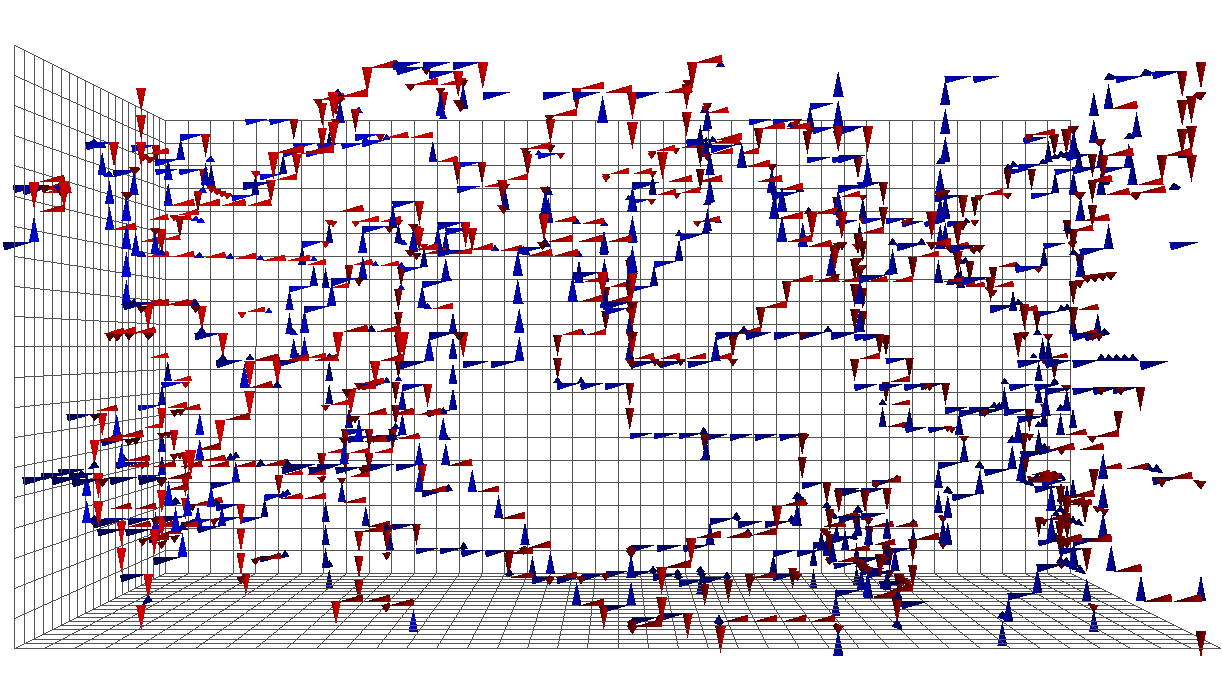
\includegraphics[width=\linewidth]{Plaq_CFG95_T01.png}
\caption{\label{fig:PlaqT01}The $t=1$ slice with all space-oriented vortices plotted.}
\end{figure}
}
%
{\centering
\begin{figure}[htb!]
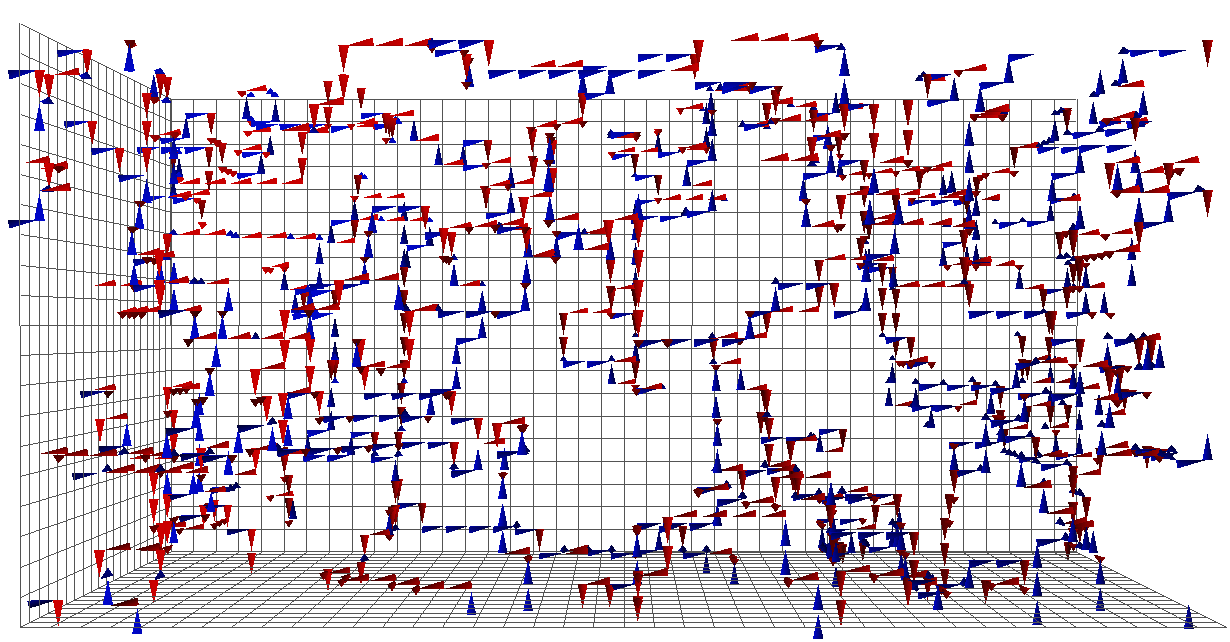
\includegraphics[width=\linewidth]{Plaq_CFG95_T02.png}
\caption{\label{fig:PlaqT02}The $t=2$ slice with all space-oriented vortices plotted.}
\end{figure}
}
%
\begin{figure}[htb!]
\centering
    \begin{subfigure}[b]{0.3\textwidth}
	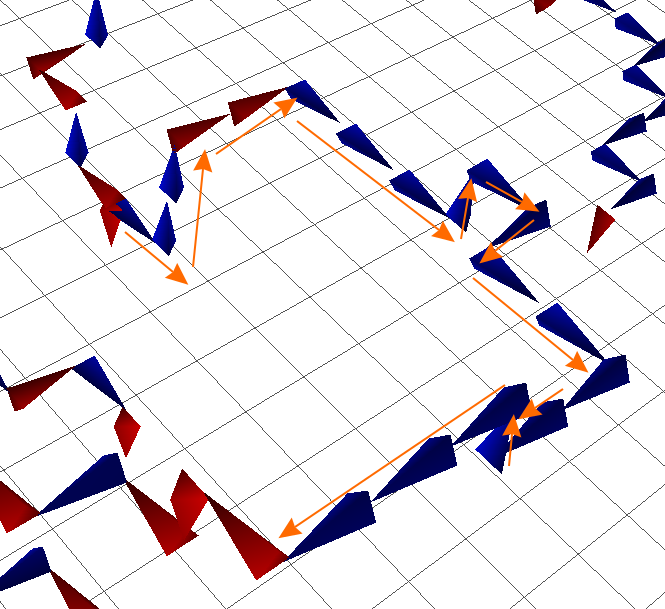
\includegraphics[width=\textwidth]{./plaqt1_line.png}
    \end{subfigure}\hfill
    \begin{subfigure}[b]{0.3\textwidth}
    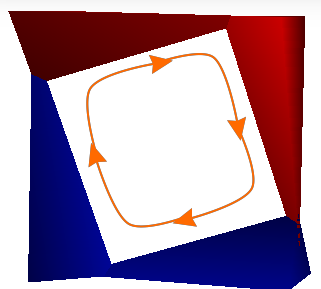
\includegraphics[width=\textwidth]{./plaqt1_loop.png}
    \end{subfigure}\hfill
    \begin{subfigure}[b]{0.3\textwidth}
	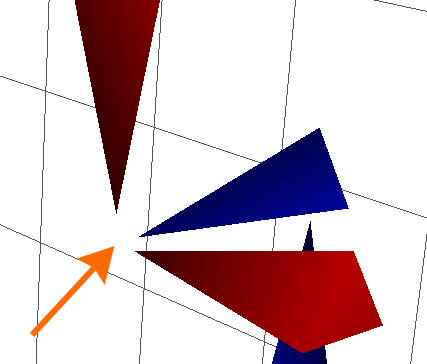
\includegraphics[width=\textwidth]{./plaqt1_monopole.png}
    \end{subfigure}
    \caption{\label{fig:VortexFeatures} \textbf{Left:} Vortices form continuous lines. Note that because of the lattice periodicity, these lines may wrap around to the opposite edge of the lattice. \textbf{Middle:} The vortices must form closed loops to conserve the vortex flux. \textbf{Right:} $SU(3)$ vortices are capable of forming monopoles or branching points where three vortices emerge or converge at a single point.}
  \end{figure}
\section{Time-Oriented Links}
\section{Topological Charge}\label{sec:TopChargeVis}
\section{Centre Vortices and Topological Charge}
